\section{Quantum bits (qubits)}

The \textit{bit} is the fundamental concept of classical computation. It has only two possible states: $0$ and $1$. Any information can be represented by a combination of bits. Using $n$ bits, a total of $2^n$ different messages can be represented/conveyed.
\\\\
Quantum computation and quantum information are built upon an analogous concept, the \textit{quantum bit}, or \textit{qubit} for short. Qubits are mathematical objects with certain properties. While it is true that qubits, like bits, are realized as actual physical systems, we are going to treat them as abstract mathematical objects.
\\\\
A qubit has a state, just like a bit, represent by $\ket{\psi}$. Two possible states are $\ket{0}$ and $\ket{1}$. However it can also have a state which is a linear combination of these two. Thus:
\begin{center}
    $\ket{\psi}=\alpha\ket{0} + \beta\ket{1}$
\end{center}

The numbers $\alpha$ and $\beta$ are complex numbers. Put another way, the state of a qubit is a vector in a two-dimensional complex vector space. The special states $\ket{0}$ and $\ket{1}$ are known as computational basis states, and form an \textit{orthonormal} basis for this vector space.
\\\\
Since $\alpha$ and $\beta$ can take infinitely many different complex values, one might be tempted to think that infinite different messages can be conveyed using a single qubit! But there's a catch. When we make a measurement of a qubit, its state \textit{collapses} into either $\ket{0}$ with probability $|\alpha|^2$ or $\ket{0}$ with probability $|\beta|^2$. So every time we observe only one of the two possible states. Naturally, $|\alpha|^2 + |\beta|^2 = 1$. 
\\\\
Geometrically, we can interpret this as the condition that the qubit’s state be normalized to length $1$. Thus, in general a qubit’s state is a unit vector in a two-dimensional complex vector space.
\\\\
Since $\alpha$ and $\beta$ are complex numbers with the only constraint that $|\alpha|^2 + |\beta|^2 = 1$, we may represent the state of qubit as:
    $$\ket{\psi} = e^{i\gamma}\left(\cos{\frac{\theta}{2}}\ket{0} + e^{i\phi}\sin{\frac{\theta}{2}}\ket{1}\right)$$

In fact, we can ignore the factor $e^{i\gamma}$ because it has no observable effects. Thus we can effectively write:
    $$\ket{\psi} = \cos{\frac{\theta}{2}}\ket{0} + e^{i\phi}\sin{\frac{\theta}{2}}\ket{1}$$

The numbers $\theta$ and $\phi$ define a point on the unit three-dimensional sphere, as shown in the figure below. This sphere is often called the \textit{Bloch sphere}.
\begin{figure}[h]
    \centering
    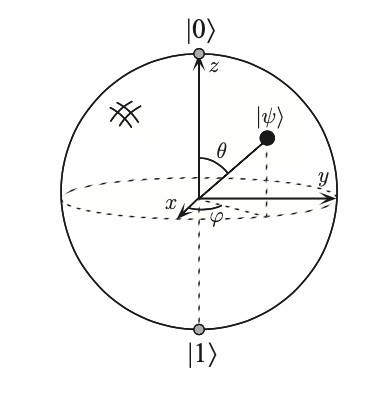
\includegraphics[width=0.35\textwidth]{bloch.png}
    \caption{Bloch sphere}
\end{figure}
